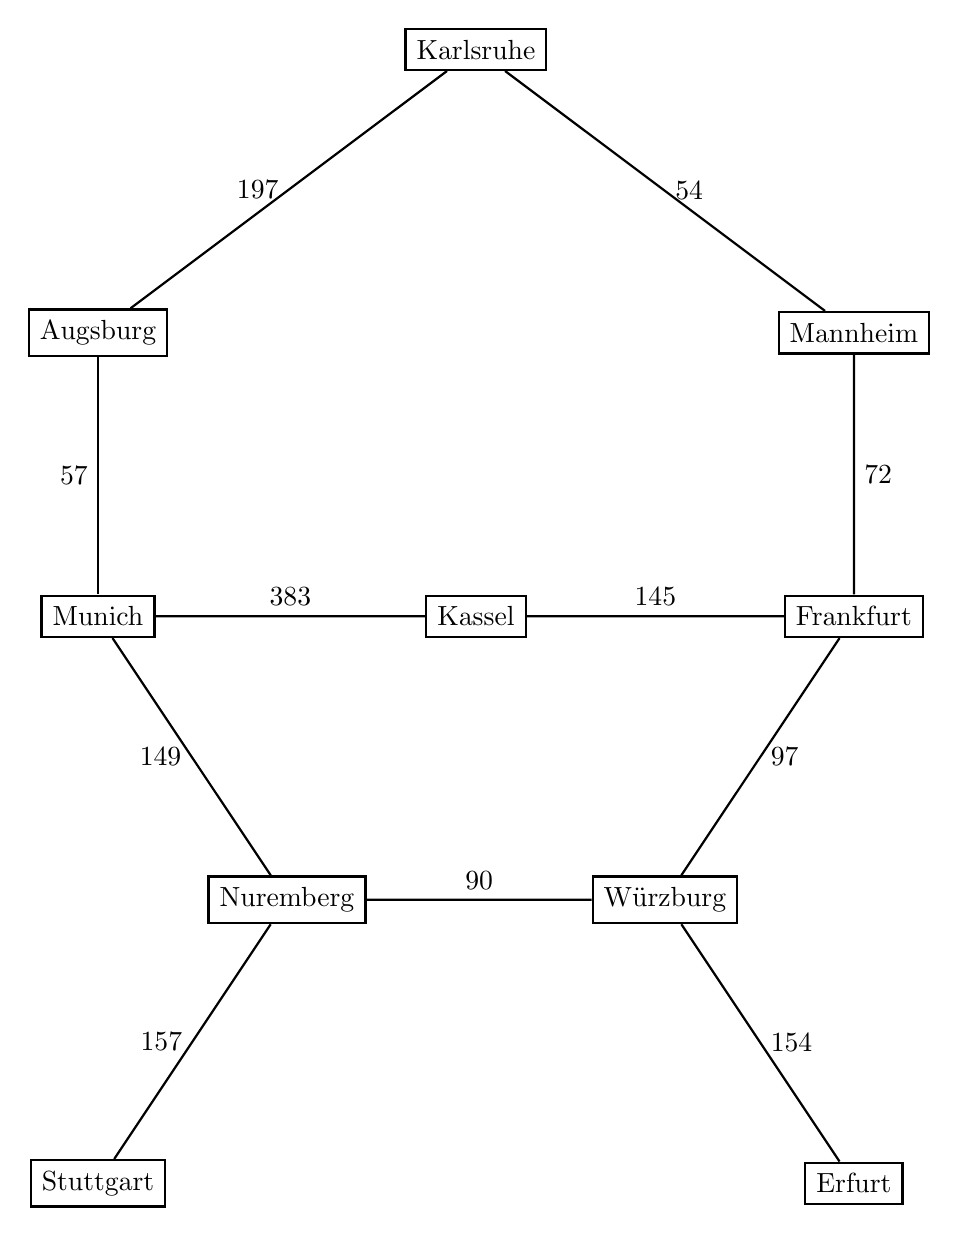
\begin{tikzpicture}
[nodedecorate/.style={shape=rectangle,inner sep=4pt,draw,thick},%
 linedecorate/.style={-,thick},%
 scale=1.2]
%% nodes or vertices
\foreach \nodename/\x/\y in {Stuttgart/0/0, Erfurt/8/0, Nuremberg/2/3,
  Munich/0/6, Frankfurt/8/6, Kassel/4/6, Augsburg/0/9, Mannheim/8/9,
  Karlsruhe/4/12}
{
  \node (\nodename) at (\x,\y) [nodedecorate] {\nodename};
}
\node (Wurzburg) at (6,3) [nodedecorate] {W\"urzburg};
%% edges or lines
\path
\foreach \startnode/\endnode/\position/\distance in {
  Stuttgart/Nuremberg/left/157, Erfurt/Wurzburg/right/154,
  Nuremberg/Wurzburg/above/90, Nuremberg/Munich/left/149,
  Wurzburg/Frankfurt/right/97, Munich/Kassel/above/383,
  Frankfurt/Kassel/above/145, Munich/Augsburg/left/57,
  Frankfurt/Mannheim/right/72, Augsburg/Karlsruhe/left/197,
  Mannheim/Karlsruhe/right/54}
{
  (\startnode) edge[linedecorate] node[\position] {\distance} (\endnode)
};
\end{tikzpicture}
